% Draft for ISMB/ECCB 2027 (proceedings, Bioinformatics). Uses article class so it builds anywhere;
% port to the OUP Bioinformatics template (9-page limit) before submission.
\documentclass[10pt,twocolumn]{article}
\usepackage[margin=0.7in]{geometry}
\usepackage{amsmath,amssymb,amsthm,booktabs,graphicx,natbib,url,xcolor}
\usepackage[T1]{fontenc}
\usepackage{microtype}
\bibliographystyle{abbrvnat}
\setcitestyle{authoryear,round}
\newcommand{\calibLo}{0.044}
\newcommand{\calibHi}{0.054}
\newcommand{\nullFDR}{0.096}
\newcommand{\advOldMax}{0.53}
\newcommand{\advOldNoDropHi}{0.20}
\newcommand{\advNewNoDropLo}{0.058}
\newcommand{\advNewNoDropHi}{0.112}
\newcommand{\advNewDropHi}{0.38}
\newcommand{\nExtCalibLo}{0.048}
\newcommand{\nExtCalibHi}{0.053}
\newcommand{\nModules}{39}
\newcommand{\nDiscovered}{0}
\newcommand{\bestP}{0.010}
\newcommand{\bhThresh}{0.0026}
\newcommand{\nBelow}{2}
\newcommand{\ksP}{0.13}
\newcommand{\nReplicated}{5}
\newcommand{\expReplicated}{3.8}
\newcommand{\nDisc}{543}
\newcommand{\nSeal}{466}
\newcommand{\nICI}{1009}
\newcommand{\nCtrl}{187}


\newtheorem{proposition}{Proposition}
\newtheorem{lemma}{Lemma}
\newcommand{\E}{\mathbb{E}}
\newcommand{\indep}{\perp\!\!\!\perp}

\title{Exact conditional module tests with external dependence structure for replicable response biology in small immunotherapy cohorts}
\author{Eshaan Nidee}
\date{Draft, \today}

\begin{document}
\maketitle

\begin{abstract}
\noindent Public immune-checkpoint-inhibitor (ICI) cohorts provide tumour transcriptomes for only 25--300 patients each. That is too few to estimate the gene--gene dependence that conditional inference requires, and response is often confounded with batch structure. Consequently, transcriptomic predictors of response rarely replicate. We present a framework that learns dependence structure (a sparse gene graph and latent-factor directions) once from large unlabelled external data, and eliminates all cohort-specific parameters by conditioning rather than estimation. The resulting gene-module test is exact in finite samples for any outcome distribution whenever the external structure contains the cohort's true structure. Evidence is combined across cohorts by a direction-consistent partial-conjunction procedure with false discovery rate (FDR) control. We show that misspecified structure induces an omitted-variable bias whose effect on FDR grows with sample size, and we neutralise it by over-spanning the external factor space. In simulations the test is calibrated in every setting and costs little power relative to an oracle, whereas marginal module tests and label-aware batch correction inflate FDR up to 2.8- and 4.5-fold. Under adversarial misspecification, over-spanning restores FDR to \advNewNoDropLo--\advNewNoDropHi. In a pre-registered, hash-sealed analysis of \nICI\ patients across ten ICI cohorts, no module carried response information beyond the established T-effector/IFN-$\gamma$ signature, and discovery $p$-values were consistent with the global null. These results establish a leakage-free standard for conditional biomarker discovery in small cohorts. They also indicate that, at current cohort sizes, T-cell inflammation accounts for the detectable transcriptomic signal of ICI response.

\medskip\noindent\textbf{Keywords:} conditional independence testing; false discovery rate control; immune checkpoint inhibitors; transcriptomic biomarkers; replicability; partial conjunction testing; external data integration; Gaussian graphical models; batch effects; pre-registration.

\medskip\noindent\textbf{Availability:} Code, simulations, the protocol and label hashes: [repository URL].
\end{abstract}

\section{Introduction}

Many studies have proposed transcriptomic predictors of response to immune checkpoint blockade. Few hold up in independent cohorts. Three features of the public data explain much of this.
\begin{itemize}
  \item \textbf{Small cohorts.} Typical cohorts have 25--300 patients and 20{,}000 genes \citep{hugo2016,riaz2017,gide2019,liu2019,jung2019,mariathasan2018,mcdermott2018,braun2020}.
  \item \textbf{Response is entangled with batch:} drug, regimen, prior therapy, biopsy site and trial.
  \item \textbf{Leakage.} Cross-cohort batch correction that protects the outcome as a covariate inflates downstream significance \citep{nygaard2016batch}.
\end{itemize}

Model-X knockoffs \citep{candes2018panning} and their multi-environment and derandomised extensions \citep{li2022multienv,ren2024derandomised} control FDR for conditional associations. They need the joint distribution of the features, or a covariance estimate that is unavailable at $n \ll p$. Conditioning on sufficient statistics removes unknown parameters \citep{huang2020relaxing}, and summary-statistic knockoffs borrow dependence structure from reference panels \citep{he2022ghostknockoff}.

We first combined the two ideas, using conditional knockoffs on an externally learned graph, with derandomised e-values and a partial-conjunction combination. Oracle simulations killed this design. With knockoffs built from the \emph{true} model, the pipeline made zero discoveries in all 288 settings we ran (cohorts of 25 to 300 patients, AUC up to 0.92). With 10--20 non-null features, knockoff+ cannot reach the minimum number of selections it needs. That result redirected us to per-hypothesis tests, which have no such floor.

\paragraph{Contributions.}
\begin{enumerate}
  \item An exact conditional test for a gene set, using an external graph and external factor directions, valid for any outcome distribution (Proposition~\ref{prop:exact}).
  \item A direction-consistent Stouffer partial-conjunction combiner across cohorts (Lemma~\ref{lem:pc}).
  \item A characterisation of how structure misspecification inflates FDR. The bias is fixed while the standard error shrinks, so inflation grows like $\sqrt{n}$ (Proposition~\ref{prop:bias}). We give a practical remedy, over-spanning, validated under adversarial stress.
  \item Simulation evidence that label-aware batch correction and marginal module tests do not control FDR for this estimand.
  \item A pre-registered, hash-sealed real-data analysis with a sealed replication audit. It gives an informative null.
\end{enumerate}

\section{Methods}

\subsection{Setting and estimand}

Cohort $k$ has $n_k$ patients with expression $X\in\mathbb{R}^{n_k\times p}$, a binary response $Y$, and cohort-internal batch labels. A pre-specified marker set $B$ (T-effector/IFN-$\gamma$ genes; \citealp{ayers2017ifng}) is never tested. For a gene set $G$ disjoint from $B$, the null is
\[
H_{G,k}:\ Y \indep X_G \mid X_{-G},\ \text{batch} \quad \text{in cohort } k .
\]
In words, the module carries no response information beyond all other measured genes, including the T-effector genes. This is deliberately stronger than marginal association. Infiltration-driven co-expression makes almost every immune module marginally associated with response.

\subsection{Exact conditional test}

Assume the rows are i.i.d. with
\[
X = F\Lambda^\top + \text{batch effects} + E, \qquad E\sim N(0,\Omega^{-1}),
\]
where $F$ holds latent factors and $\Omega$ is supported on a sparse graph. The precision of $X$ is then $\Omega$ minus a rank-$k$ term built from $W=\Omega\Lambda$. The conditional mean of $X_G$ given $X_{-G}$ is therefore linear in the design
\[
D_G=\bigl[\,1,\ \text{batch},\ X_{N(G)},\ X_{-G}W_{-G}\,\bigr],
\]
where $N(G)$ is the graph neighbourhood of $G$ outside $G$. The conditional error is homoscedastic Gaussian. The coefficients and the residual covariance are cohort-specific and unknown, but they never need to be estimated.

\begin{proposition}\label{prop:exact}
Let $r=r(Y,X_{-G},\text{batch})$ be any residual, for example $Y$ minus its least-squares fit on batch and the marker-set mean. Let $T$ be the Wilks statistic for adding $r$ to the multivariate regression of $X_G$ on $D_G$. Assume the external graph contains $N(G)$ and $\mathrm{span}(W_{-G})$ contains the true factor span. Then under $H_{G,k}$,
\[
\tfrac{1-T}{T}\cdot\tfrac{n-q-g}{g}\ \sim\ F_{g,\,n-q-g},
\]
where $g=|G|$ and $q=\mathrm{rank}(D_G)$, whatever the conditional law of $Y$.
\end{proposition}
\begin{proof}[Proof sketch]
Under $H_{G,k}$ with independent rows, the law of $X_G$ given $(X_{-G},Y,\text{batch})$ equals its law given $(X_{-G},\text{batch})$. That is the Gaussian linear model $X_G=D_G\beta+\mathcal{E}$, whose rows are i.i.d. $N(0,\Sigma_c)$. Both $D_G$ and $r$ are fixed under this conditioning, and the true coefficient on $r$ is zero. The classical one-regressor multivariate test gives the exact $F$ law. It is invariant to $\beta$ and $\Sigma_c$, and to any nonsingular transformation $X_G\mapsto X_GA$.
\end{proof}

The primary statistic projects $X_G$ onto its mean, a fixed direction, which gives an exact $t$-test with $n-q-1$ degrees of freedom. We report it as a signed $z$-score, $z=\Phi^{-1}(F_t(t))$.

Only $N(\cdot)$ and $W$ come from outside the cohort. Means, coefficients, covariance and batch shifts are all conditioned away. Gene scaling is fixed from the external data, so no cohort statistic of $X_G$ enters the design.

\subsection{External structure, and inflating it}

From unlabelled expression of the matched tumour types (TCGA; \citealp{tcga2013pancan}):
\begin{itemize}
  \item standardise each gene;
  \item estimate $k$ principal factors;
  \item fit a neighbourhood-lasso graph to the factor residuals \citep{meinshausen2006}, take its union with each gene's top correlation partners, and cap the degree;
  \item estimate $\Omega$ on that graph.
\end{itemize}

Proposition~\ref{prop:exact} requires \emph{containment} of the true structure, not exact recovery. We therefore inflate both parts.
\begin{itemize}
  \item \textbf{Graph:} the union with correlation partners adds edges.
  \item \textbf{Factor span:} we use $W=[\hat\Omega\hat\Lambda,\ \hat\Lambda]$ with an over-specified $k$.
\end{itemize}
Each extra column costs one degree of freedom. We fix $k=\mathrm{clip}(\lfloor n/25\rfloor,2,8)$ and skip a module in a cohort if fewer than 8 residual degrees of freedom remain.

\subsection{Combining cohorts}

Replicability is framed as a partial conjunction: $H^{r/K}_G$ says that $G$ is non-null in fewer than $r$ of $K$ cohorts \citep{benjamini2008pc}.

\begin{lemma}\label{lem:pc}
Suppose the cohorts are independent. For each sign $s \in \{+1,-1\}$, let $p^{(s)}_{(1)}\le\dots\le p^{(s)}_{(K)}$ be the ordered one-sided $p$-values $1-\Phi(s z_k)$. Then
\[
P^{r/K}_G = \min\Bigl\{1,\ 2\min_{s}\ \bar\Phi\Bigl(\textstyle\sum_{i\ge r}\Phi^{-1}\bigl(1-p^{(s)}_{(i)}\bigr)/\sqrt{K-r+1}\Bigr)\Bigr\}
\]
is a valid $p$-value for $H^{r/K}_G$.
\end{lemma}

Validity of combining the $K-r+1$ largest $p$-values follows from \citet{benjamini2008pc}. The factor of two is a Bonferroni correction over the two signs. We apply BH \citep{benjamini1995} across modules. Independence across cohorts is a correctness requirement, so we screen for duplicate patients (Section~\ref{sec:data}).

\subsection{Misspecification and why inflation grows with $n$}

\begin{proposition}\label{prop:bias}
Suppose the true conditional mean contains a term $U\gamma$, with $U=X_{-G}c\notin\mathrm{span}(D_G)$. This happens when an edge is missing or the factor span is under-estimated. Then under $H_{G,k}$ the $t$-statistic for $r$ has non-centrality
\[
\delta_n \approx \sqrt{n}\,\gamma\,\mathrm{Cov}(r,U\mid D_G)\big/\bigl(\sigma_c\,\mathrm{sd}(r\mid D_G)\bigr).
\]
\end{proposition}

This is the usual omitted-variable calculation. It is non-zero only when the omitted direction is correlated with the outcome residual, which is exactly what happens when it touches a response-relevant gene. The bias is fixed while the standard error shrinks, so FDR inflation \emph{grows} with $n$. This matches the simulations below. It motivates over-spanning, and it explains why correlated nuisance biology is the dangerous case rather than random missing edges.

\subsection{Pre-registration}

All label-free choices were frozen in a protocol and committed before any outcome was read:
\begin{itemize}
  \item gene universe, marker set and module recipe;
  \item batch variables and response definitions;
  \item sealed cohorts, primary analysis and replication rule.
\end{itemize}
The commit includes SHA-256 hashes of every label file. The analysis script refuses to read true labels unless the protocol is committed and every hash matches.

\section{Simulations}

\paragraph{Design.} Each simulated dataset has:
\begin{itemize}
  \item 520 genes: 50 tested modules of 10, plus 20 marker genes whose mean drives response;
  \item AR(1) residual dependence within modules, and four latent factors, one of them diffuse;
  \item a two-level batch with gene-specific shifts and a response-rate shift;
  \item binary $Y$ with heterogeneous effects across cohorts.
\end{itemize}
Signal is either \emph{sparse} (2 genes per module, random signs) or \emph{coherent} (all genes in a module, one sign). Effect sizes are calibrated by the AUC of the signal genes' combined score, 0.65--0.80, the range reported for ICI signatures. External structure is learned from $N_{\rm ext}=2000$ or $500$ unlabelled samples. All results use $K=6$ cohorts, BH at $\alpha=0.1$ and $r=1$ unless stated, with 50--500 replicates per cell.

\paragraph{Calibration and power.} Across all settings, the rejection rate of null modules at level 0.05 was \calibLo--\calibHi\ with oracle structure, and \nExtCalibLo--\nExtCalibHi\ with structure learned from $N_{\rm ext}=500$. A 500-replicate global-null check gave FDR \nullFDR.

Fig.~\ref{fig:power} shows power with oracle structure. For coherent signal at AUC 0.75, power is 0.51 at $n=100$ and 0.99 at $n=300$. Learning the structure externally kept most of this: 0.37--0.50 at $n=100$ and 0.96--0.98 at $n=300$. Requiring replication ($r=2$) is far costlier below $n\approx300$. Single-gene tests had almost no power, so modules are the inferential unit.

\begin{figure}[t]
\centering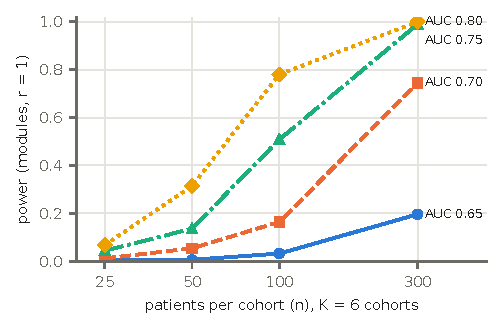
\includegraphics[width=\columnwidth]{figs/fig_power.pdf}
\caption{Power of the conditional module test with oracle structure (coherent signal, $K=6$, $r=1$). Power is limited below $n\approx100$ per cohort, even at the oracle.}
\label{fig:power}
\end{figure}

\paragraph{Baselines.} Table~\ref{tab:baselines} and Fig.~\ref{fig:baselines} compare five methods on identical cohorts whose response rates differ, as objective response rates do across tumour types. Only the conditional tests controlled FDR.
\begin{itemize}
  \item Marginal per-cohort tests absorb shared infiltration, so their FDR grows with $n$.
  \item Pooling with label-aware correction (a ComBat-style protected covariate; \citealp{johnson2007combat}) inflated FDR even under the global null. Its label-blind counterpart did not under the global null, which is the leakage mechanism of \citet{nygaard2016batch}. With signal present, both pooled variants inflate, like the marginal test, because none conditions on the other modules.
  \item In-sample structure was valid but less powerful at $n=100$ (0.21 against 0.34).
\end{itemize}

\begin{table}[t]
\centering\footnotesize
\caption{FDR and power on the same simulated cohorts ($K=6$, 50 replicates). $^a$Mean over $n\in\{50,100,300\}$ with no signal.}
\label{tab:baselines}
\resizebox{\columnwidth}{!}{\begin{tabular}{lccccc}
\toprule
 & \multicolumn{3}{c}{FDR (coherent, AUC 0.75)} & FDR & Power \\
Method & $n{=}50$ & $n{=}100$ & $n{=}300$ & global null$^a$ & $n{=}300$ \\
\midrule
\textbf{Ours (external structure)} & 0.087 & 0.071 & 0.086 & 0.120 & 0.96 \\
In-sample structure & 0.035 & 0.109 & 0.089 & 0.107 & 0.94 \\
Marginal per cohort & 0.154 & 0.164 & 0.281 & 0.100 & 0.88 \\
Pooled, label-aware correction & 0.268 & 0.257 & 0.448 & 0.207 & 0.83 \\
Pooled, label-blind correction & 0.097 & 0.123 & 0.278 & 0.073 & 0.87 \\
\bottomrule
\end{tabular}
}
\end{table}

\begin{figure*}[t]
\centering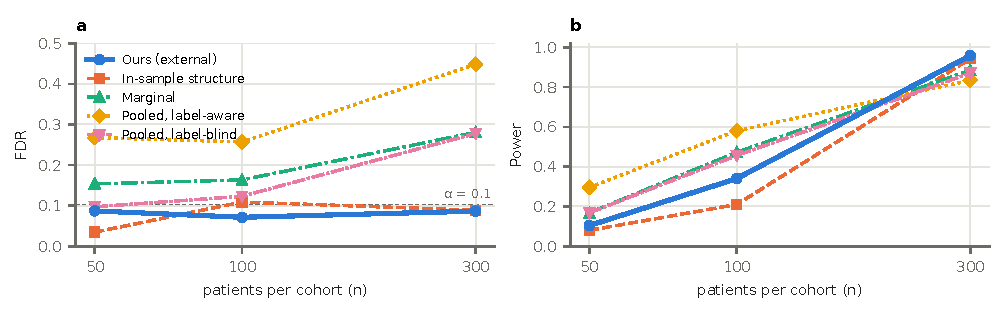
\includegraphics[width=0.8\textwidth]{figs/fig_baselines.pdf}
\caption{(a) FDR and (b) power by method (coherent signal, AUC 0.75). Dotted line: nominal $\alpha$. Methods with higher power at small $n$ achieve it in cells where their FDR is inflated.}
\label{fig:baselines}
\end{figure*}

\paragraph{Adversarial stress test.} We added 40 true edges joining signal genes to genes in null modules (partial correlation 0.25), the worst case under Proposition~\ref{prop:bias}, and deleted a fraction of them from the learned graph (Fig.~\ref{fig:adversarial}).
\begin{itemize}
  \item With $k=4$ and $W=\hat\Omega\hat\Lambda$, FDR reached \advOldNoDropHi\ at $n=300$ \emph{with nothing deleted}, and \advOldMax\ with all deleted.
  \item With oracle structure, FDR was 0.10. So the inflation came from estimation error in $W$, not from the test.
  \item Distilling the outcome residual with a lasso on $X_{-G}$ \citep{liu2022dcrt} did not help.
  \item Over-spanning ($k=8$, $W=[\hat\Omega\hat\Lambda,\hat\Lambda]$) restored FDR to \advNewNoDropLo--\advNewNoDropHi\ with nothing deleted. Power was unchanged at $n=300$, and lower at $n=100$ (0.12 against 0.20).
  \item When true edges are deleted, inflation remains, up to \advNewDropHi. No cohort-internal procedure can recover an omitted direction without a label-dependent choice of design.
\end{itemize}

\begin{figure*}[t]
\centering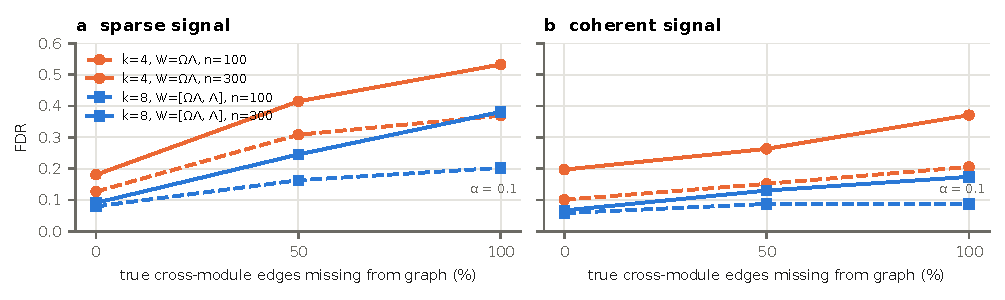
\includegraphics[width=0.8\textwidth]{figs/fig_adversarial.pdf}
\caption{FDR under adversarial missing edges (AUC 0.8). Orange: default factor directions. Blue: over-spanned. Solid $n=300$, dashed $n=100$. Inflation grows with $n$, as Proposition~\ref{prop:bias} predicts.}
\label{fig:adversarial}
\end{figure*}

\section{Real data}\label{sec:data}

\paragraph{Cohorts.} The cohorts are listed in Table~\ref{tab:cohorts}.
\begin{itemize}
  \item \textbf{Sources:} GEO (Hugo, Riaz, Jung, GSE176307; \citealp{gse176307}); iAtlas-harmonised cBioPortal studies (Gide, Liu, IMvigor210, IMmotion150; \citealp{iatlas,cerami2012cbioportal}); and the Braun supplementary tables.
  \item \textbf{Labels:} response is CR/PR against SD/PD. Jung has no RECIST data in GEO, so we used durable clinical benefit (PFS $\ge$180 days). Samples are pre-treatment, one per patient.
  \item \textbf{Batch:} cohort-internal batch variables follow the protocol.
  \item \textbf{External structure:} learned per cohort from matched TCGA tumour types.
  \item \textbf{Modules:} the fixed recipe produced \nModules\ modules covering about 400 of 1500 high-variance genes.
\end{itemize}

\textbf{Duplicate screen.} Each gene is ranked within its cohort, five principal components are removed, and samples are correlated across cohorts. We calibrated this on a positive control: Hugo from GEO against the iAtlas re-processing, the same 26 patients through different pipelines. True pairs scored $\rho\ge0.67$, non-pairs $\le0.27$, and impossible NSCLC--ccRCC pairs $\le0.28$. Ten pairs crossed the threshold of 0.5. None was plausible as a shared patient, and all 14 samples involved were excluded by the pre-specified rule.

\paragraph{Design.} Eight cohorts (\nDisc\ patients) were used for discovery. IMvigor210 and Braun nivolumab (\nSeal\ patients) were sealed for replication. The sunitinib and everolimus arms (\nCtrl\ patients) were descriptive controls.

\begin{table}[t]
\centering\footnotesize
\caption{Cohorts after duplicate exclusion.}
\label{tab:cohorts}
\resizebox{\columnwidth}{!}{\begin{tabular}{llrrcc}
\toprule
Cohort & Tumour & $n$ & Resp. & Role & Batch \\
\midrule
Hugo 2016 & melanoma & 26 & 14 & discovery & -- \\
Riaz 2017 & melanoma & 49 & 10 & discovery & -- \\
Gide 2019, PD-1 & melanoma & 41 & 19 & discovery & -- \\
Gide 2019, ipi+PD-1 & melanoma & 32 & 21 & discovery & -- \\
Liu 2019 & melanoma & 121 & 47 & discovery & prior anti-CTLA-4 \\
Jung 2019 & NSCLC & 27 & 7 & discovery & -- \\
GSE176307 & urothelial & 87 & 16 & discovery & IO line \\
IMmotion150, atezo $\pm$ bev & ccRCC & 160 & 48 & discovery & bevacizumab \\
IMvigor210 & urothelial & 298 & 68 & sealed & biopsy site \\
Braun 2020, nivolumab & ccRCC & 168 & 38 & sealed & trial \\
IMmotion150, sunitinib & ccRCC & 81 & 24 & control & -- \\
Braun 2020, everolimus & ccRCC & 106 & 5 & control & -- \\
\bottomrule
\end{tabular}
}
\end{table}

\paragraph{Pre-registered result.} There were \nDiscovered\ discoveries at $r=1$, at $r=2$, and with Simes. The marginal and pooled label-aware baselines also made none.
\begin{itemize}
  \item The strongest module, the metallothioneins MT1G/A/H/M/E, had $P=\bestP$. A single BH rejection would require $P\le\bhThresh$. Its evidence was positive in 7 of 8 discovery cohorts but negative in both sealed cohorts.
  \item Discovery $p$-values were consistent with uniform: \nBelow\ of \nModules\ were below 0.05, and the Kolmogorov--Smirnov test against uniform gave $p=\ksP$ (Fig.~\ref{fig:real}a).
  \item Sealed-cohort ``replication'' occurred for \nReplicated\ of \nModules\ modules, against \expReplicated\ expected by chance.
\end{itemize}

\paragraph{Exploratory check (post-unsealing).} To rule out broken labels or a broken pipeline, we computed the AUC of the marker-set mean (Fig.~\ref{fig:real}b).
\begin{itemize}
  \item It was predictive in Gide (both regimens), Jung, IMmotion150 and IMvigor210.
  \item It was null in both non-ICI controls.
  \item It was null in Braun nivolumab and Hugo, as those studies reported for infiltration and IFN signatures \citep{braun2020,hugo2016}.
\end{itemize}
The labels and pipeline therefore behave as the literature predicts. The confirmatory null concerns information \emph{beyond} this score.

\begin{figure*}[t]
\centering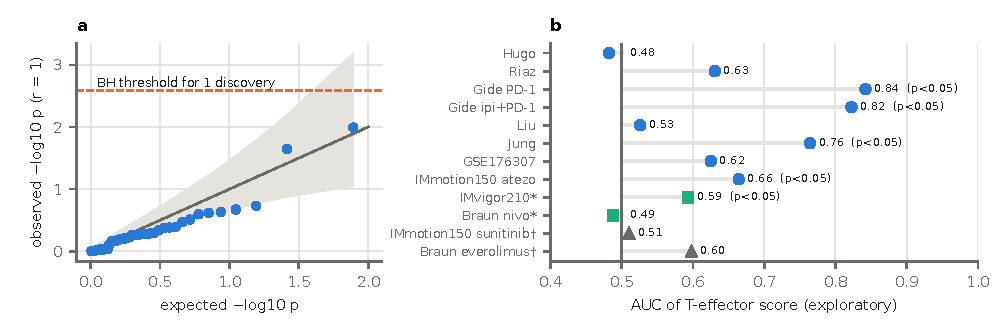
\includegraphics[width=0.8\textwidth]{figs/fig_real.pdf}
\caption{(a) QQ plot of pre-registered discovery $p$-values ($r=1$, \nModules\ modules) with a 95\% band. Dashed line: BH threshold for one discovery. (b) Exploratory AUC of the T-effector score. Circles: discovery. Squares (*): sealed. Triangles (\dag): non-ICI controls.}
\label{fig:real}
\end{figure*}

\section{Discussion}

The method separates what small cohorts can supply from what they cannot. External data supply the dependence structure. The cohort's own nuisance parameters are conditioned away exactly. The guarantee holds for any outcome model and depends only on containment of the true structure. That shifts the burden to the external structure. Our stress tests show where this assumption bites: in correlated nuisance biology, with inflation that grows with $n$. They also show that over-spanning is a cheap, effective guard.

The real-data null is informative. With \nICI\ patients, an estimand that conditions on T-cell inflammation, and a design that cannot leak, no module of a fixed TCGA-derived set added detectable response information. This is consistent with the dominance of T-cell inflammation in ICI response, and with the poor transfer of richer signatures. Methods without conditional control would have reported discoveries in our simulations under the same conditions.

\paragraph{Limitations.}
\begin{itemize}
  \item Exactness assumes conditional Gaussianity on the log scale. Robustness to RNA-seq marginals needs further study.
  \item The module recipe covers a minority of genes.
  \item Power below about 100 patients per cohort is low even at the oracle.
  \item Missing edges that touch response-relevant genes cannot be repaired. A formal bound in terms of missing-edge mass remains open.
  \item The Braun expression matrix was used as released by the authors.
  \item The estimand is conditional association, not causation or clinical utility.
\end{itemize}

\section*{Acknowledgements}
[To be added.]

\bibliography{refs}
\end{document}
